\section{Implementation}\label{sec:implementation}

In the following sections the main steps of the implementation will be presented. The C++ source code along with the complete results are available at \footnote{\url{https://github.com/carlosmccosta/Currency-Recognition}}. To speed up development, the \gls{opencv} library was used.


\subsection{Preprocessing}

To improve the detection of good features and ensure that the system has robust recognition even when the images have considerable noise, a preprocessing step is applied.

In a first phase, most of noise is removed using a bilateral filter \cite{Tomasi1998}. This filter was chosen because it preserves the edges of the image blobs, which are very valuable structures in the detection of feature points.

After the noise is reduced, a \gls{clahe} \cite{Heckbert1994} is applied to increase the contrast. This can improve the recognition of the system when the images are taken in low light environments. This technique has better results over the simple histogram equalization because it can be applied to images that have areas with high and low contrast, and also limits the spread of the noise.

Finally, the brightness is adjusted to correct images that are too dark or too bright.

\Cref{fig:preprocessing} shows the impact of the preprocessing stage in an image which had noise caused by the wrinkled plastic.

\begin{figure}[H]
	\centering
	\begin{minipage}[h]{.498\textwidth}
		\centering
		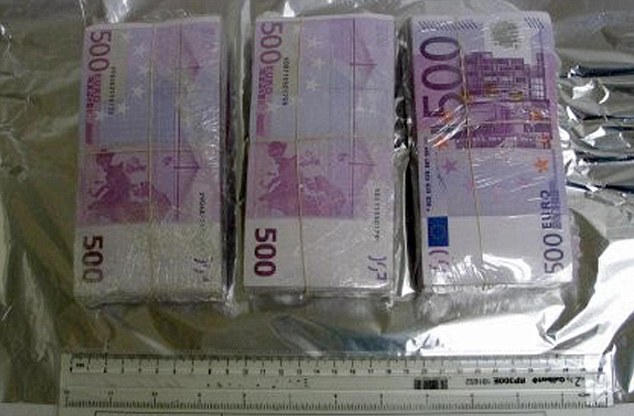
\includegraphics[width=\textwidth]{preprocessing/before-500-500-500}
	\end{minipage}\hfill
	\begin{minipage}[h]{.498\textwidth}
		\centering
		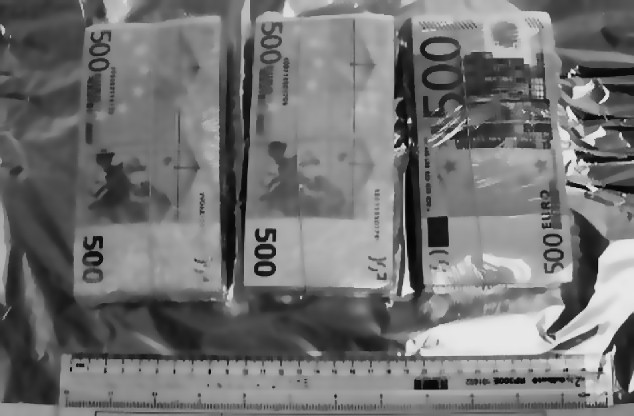
\includegraphics[width=\textwidth]{preprocessing/after-500-500-500}
	\end{minipage}
	\caption{Impact of preprocessing stage (original image on the left, preprocessed image on the right)}
	\label{fig:preprocessing}
\end{figure}


\subsection{Reference image database setup}

In order for the system to be able to recognize the target banknotes, a database of valid instances must be computed.

This database contains the descriptors associated with the keypoints for each banknote (from both sides). These descriptors are calculated in the same way as presented in section \cref{sec:feature-detection} and \cref{sec:keypoint-descriptor-extraction} and the images are also preprocessed.

To improve the detection of the relevant parts of the banknotes and to avoid the usage of sections that are similar across several banknotes, the keypoint detection algorithm is only applied inside the masks associated with each banknote. Only relevant parts such as the banknote number and unique textures or patterns are included in the banknotes masks (only the white areas shown in \cref{fig:banknote-feature-detection-mask-500-front} will be used to compute the keypoints).


\begin{figure}[H]
	\centering
	\begin{minipage}[h]{.498\textwidth}
		\centering
		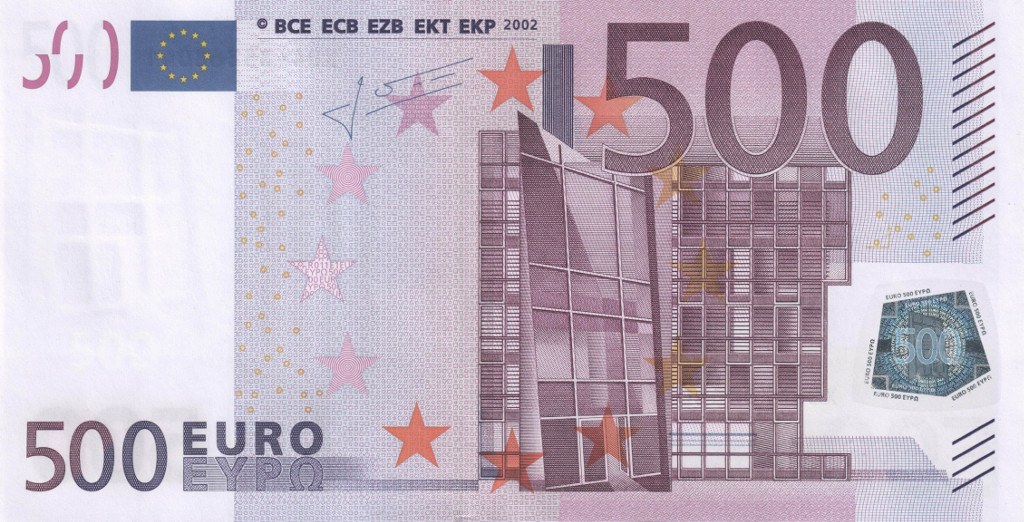
\includegraphics[width=\textwidth]{notes-masks/500eu-front}
	\end{minipage}\hfill
	\begin{minipage}[h]{.498\textwidth}
		\centering
		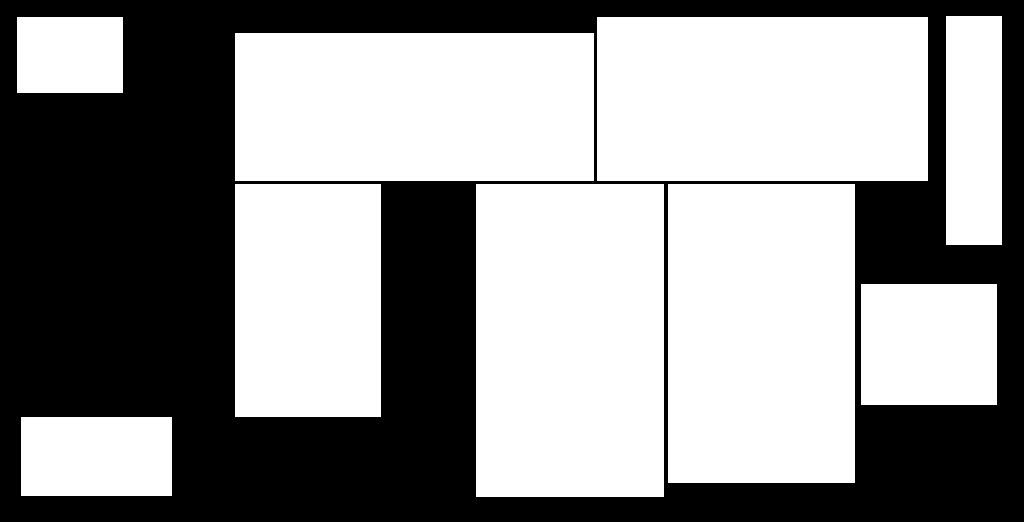
\includegraphics[width=\textwidth]{notes-masks/500eu-front-mask}
	\end{minipage}
	\caption{Front of a 500\,\euro{} banknote (left) with associated feature detection mask (right)}
	\label{fig:banknote-feature-detection-mask-500-front}
\end{figure}

%\begin{figure}[H]
%	\centering
%	\begin{minipage}[h]{.498\textwidth}
%		\centering
%		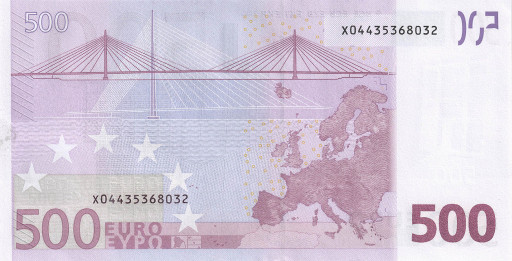
\includegraphics[width=\textwidth]{notes-masks/500eu-back}
%	\end{minipage}\hfill
%	\begin{minipage}[h]{.498\textwidth}
%		\centering
%		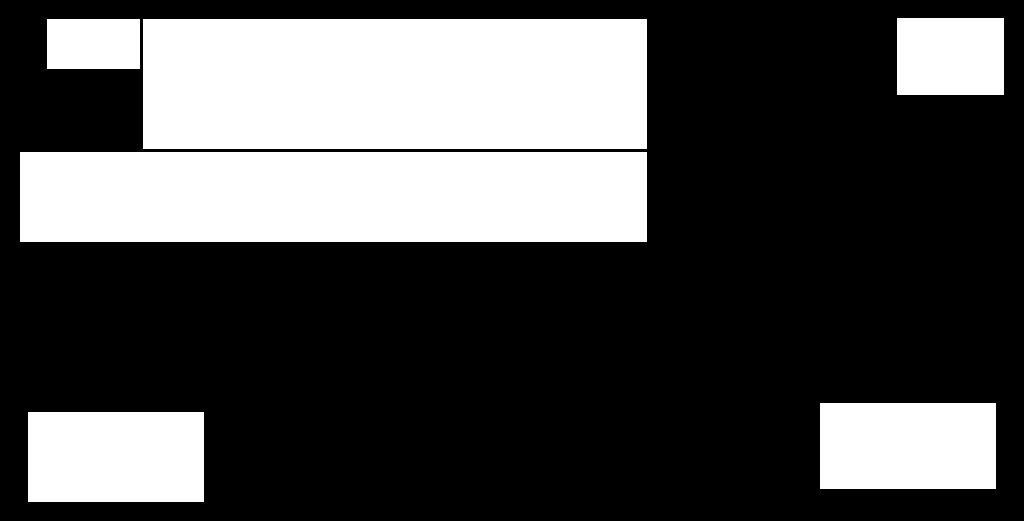
\includegraphics[width=\textwidth]{notes-masks/500eu-back-mask}
%	\end{minipage}
%	\caption{Back of a 500\,\euro{} banknote (left) with associated feature detection mask (right)}
%	\label{fig:banknote-feature-detection-mask-500-back}
%\end{figure}


\subsection{Recognition}

The recognition is the most critical phase in the system, in which the provided image is analyzed to extract the banknotes monetary value and their contour.

The current implementation supports recognition of multiple banknotes in the same image, even if they are partially occluded.

The system was implemented to recognize any type of banknotes. The Euro currency was selected for the computation of the results, but any other currency can be used. To setup the system for other currencies it is only necessary to replace the database images and masks with the intended currency images.

To improve the robustness of the system, 3 levels of detail for each banknote are provided (with images having width of 256, 512 and 1024 respectively).

For an ideal banknote recognition result, the image resolution of both the reference and the target images should be the same. But converting a high resolution banknote database to the image banknotes resolution has a considerable overhead in the system performance, and as such, to allow the system to be more efficient and able to run in real time, a compromise between precision and computation time was achieved by precomputing the reference images in 3 different scales. At run time, the appropriate level of detail is selected according to the resolution of the target image.

The reason for several levels of details is related to the fact that the geometry of the banknotes changes drastically from a very low resolution to a high resolution banknote image. As a result, the computed keypoints and their associated descriptors will be considerably different and the recognition of the banknotes will likely fail. This can be clearly seen in \cref{fig:banknote-500-front-resolution-difference}. This approach mitigates this problem by selecting the most similar database image resolution in relation to the banknotes in the image being analyzed.

\begin{figure}[H]
	\centering
	\begin{minipage}[h]{.249\textwidth}
		\centering
		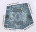
\includegraphics[width=\textwidth]{image-resolution/500eu-front-very-low}
	\end{minipage}\hfill
	\begin{minipage}[h]{.249\textwidth}
		\centering
		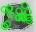
\includegraphics[width=\textwidth]{image-resolution/500eu_front_currencyDB_veryLowResolution_SIFT-Detector}
	\end{minipage}\hfill
	\begin{minipage}[h]{.249\textwidth}
		\centering
		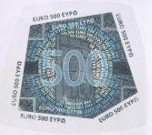
\includegraphics[width=\textwidth]{image-resolution/500eu-front-medium}
	\end{minipage}\hfill
	\begin{minipage}[h]{.249\textwidth}
		\centering
		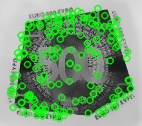
\includegraphics[width=\textwidth]{image-resolution/500eu_front_currencyDB_mediumResolution_SIFT-Detector}
	\end{minipage}
	\caption{Impact of image resolution when computing SIFT keypoints from a very low resolution image (left) to a high resolution image (right) of the hologram of a 500\,\euro{} banknote}
	\label{fig:banknote-500-front-resolution-difference}
\end{figure}


\subsubsection{Feature detection}\label{sec:feature-detection}
Feature detection is the initial recognition step in which interesting keypoints for matching are identified in the image.

These keypoints are normally selected by analyzing the edges, corners, blobs or even ridges. Also, the keypoints provide a condensed representation of the image, which significantly speeds up matching (compared to bitmap or blob matching).

To allow fine tuning of the system, the implementation supports the usage of several feature detection algorithms. Namely, \gls{sift} \cite{Lowe2004}, \gls{surf} \cite{Bay2006}, \gls{gftt} \cite{Shi1994}, \gls{fast} \cite{Rosten2006}, \gls{orb} \cite{Rublee2011}, \gls{brisk} \cite{Leutenegger2011}, STAR \cite{Agrawal2008} and \gls{mser} \cite{Matas2004}.


\subsubsection{Keypoint descriptor extraction}\label{sec:keypoint-descriptor-extraction}

The feature description step associates to each keypoint a description of its surroundings, in order to allow the matching of keypoints. This normally involves the computation of n-jets or local histograms and the final result is a vector in an n-dimensional space characterizing each keypoint.

In order to detect instances with different perspective views, these descriptors must be scale and rotation invariant. Also, they should tolerate different lightning conditions.

There are several algorithms that can accomplish this task, and as such, they were included in the implementation and can be selected to fine tuning the system. It was included the \gls{sift} \cite{Lowe2004}, \gls{surf} \cite{Bay2006}, \gls{freak} \cite{Alahi2012}, \gls{brief} \cite{Calonder2010}, \gls{orb} \cite{Rublee2011} and \gls{brisk} \cite{Leutenegger2011} feature descriptors.


\subsubsection{Descriptors matching and inliers filtering}\label{sec:descriptors-matching-and-inliers-filtering}

In order to detect multiple banknotes in the same image, a correct matching between the image descriptors and the reference banknotes descriptors must be establish. Moreover, these matches should be verified to see if they really belong to a banknote.

The initial matching can be performed using either a brute force or a heuristic approach.

In the brute force approach, each descriptor in the image is compared with all descriptors in the reference image to find the best correspondence.

In the heuristic approach, such as the \gls{flann} library \cite{Muja2009}, several optimizations are employed to speed up the computations. These optimizations can be related to the appropriate selection of which keypoints to match, and to the use of efficient data structures to speed up the search (such as k-d trees).

After the initial matching, an inliers filtering phase is applied. It starts by applying a ratio test (presented in section 7.1 of \cite{Lowe2004}) and then refines the results with the computation of a homography.

In the ratio test, each image keypoint descriptor is associated with the two best reference image descriptors. This allows to decide if the matching is correct or not, by computing the ratio between the distances of these references keypoints. The rationale behind it, is that if the ratio is close to 1, then there are two points with equivalent match probability, and as such, is very likely that this is an incorrect match, and should be discarded.

The refinement of the inliers is performed with the computation of a homography that allows the mapping of the positions in the reference image to the positions in the target image, in which the banknotes to be recognize reside. This is achieved by using the \gls{ransac} \cite{Fischler1981} method to find the homography that best fits the detected keypoints. Since this is a RANdom SAmple Consensus method, it iteratively tries to find better results by randomly selecting the supporting keypoints until there is a high confidence in the results or the maximum number of iterations is reached. The rationale behind using such method, is that the geometry of the banknotes is planar, and if it is assumed that in most cases the banknotes that are going to be recognize have also planar geometry, then a homography can be used to analyze if a match is correct or not. This classification is performed by applying the homography to the reference keypoints and see if the result position in the target image is close to the position of the matched keypoint. If it is, then the match can be considered correct.

Having the inliers, two approaches can be used to decide if a valid banknote was found or not.

One technique relies in the computation of the global inliers ratio in relation to the number of keypoints, and considers that there was a correct match if this ratio is above a given threshold. This is the most appropriate method for most of the cases of recognition.

Another method that may yield better results when the banknotes are partially occluded, is to considering a correct match when one of the components of the masks (shown in Fig. 1) have the local inliers ratio above a given threshold. The idea behind this approach is to consider each patch of the image represented in the mask as a unique identifier of the banknote. As such, if this local patch is correctly detected, then there is a high confidence that the recognition of that banknote was successful.


\subsubsection{Shape analysis}\label{sec:shape-analysis}

When a banknote matching is considered valid, it undergoes a postprocessing step in which its contour shape is analyzed.

This step is crucial to avoid the multiple detection of the same banknote when it is wrinkled or folded. Also, it removes any recognition that have a contour shape that can't be associated with a banknote.

The initial filtering is performed by removing any result which have a contour with a very low area in relation to the whole image.

In a second step, any result without a convex contour is also removed. This is applied because a banknote has a convex quadrilateral shape. It will never have a concave shape, even when it is folded. The reason for this is that the contour is not computed from the banknote borders. Instead a homography is used to map the 4 corners of the reference image to the positions in the image in which the banknotes reside.

A final step removes any result that has a contour with a circularity or aspect ratio outside the acceptable bounds. These bounds are retrieved from a database of valid shapes, as shown in \cref{fig:currency-db-shapes}.

\begin{figure}
	\centering
	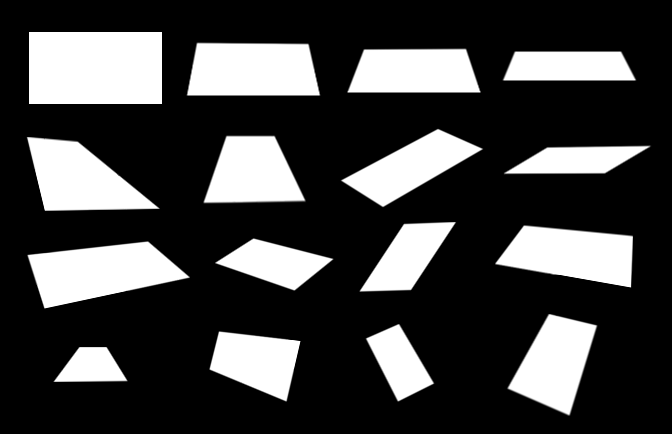
\includegraphics[width=0.46\linewidth]{notes-masks/currency-db-shapes}
	\caption{Database of valid instances of banknote shapes}
	\label{fig:currency-db-shapes}
\end{figure}


\subsubsection{Detection of multiple banknotes}

In order to recognize several banknotes in the same image, the steps presented in \cref{sec:descriptors-matching-and-inliers-filtering,sec:shape-analysis} are performed to every banknote reference image, and the best match is chosen. After the retrieval of the best match, its inliers are removed from the keypoint set, and these two steps (shown in \cref{sec:descriptors-matching-and-inliers-filtering,sec:shape-analysis}) are repeated again for every reference image, in order to find another banknote. This is done until no valid match is found.

Only the inliers must be removed from the keypoint set in order to be able to successful recognize partially occluded banknotes. A less robust method (not used), that will likely fail, removes the keypoints that are inside the banknote contour. Although it might require less computations to perform, it will fail to detect banknotes that are on top of each other, because part of their keypoints will be removed when one of the banknotes is detected.
